\documentclass[11pt]{article}
\pagestyle{plain}

\usepackage{amssymb}
\usepackage{amsmath}
\usepackage{amsfonts}
\usepackage{graphics}
\usepackage{graphicx}

\title{LINMA1170 - Devoir 1}
\author{Giovanni Karra - 45032100}

\begin{document}

\maketitle

\section{Questions théoriques}
\begin{enumerate}
    \item On sait que $||AX - B||_F^2 = tr((AX - B)^T(AX - B)) = tr(X^TA^TAX - B^TAX - X^TA^TB + B^TB)$.\\
    On sait aussi que $\nabla_X tr(AX) = tr(\nabla_X AX)$.\\
    On a donc $\nabla_X||AX - B||_F^2 = tr(2A^TAX-2A^TB) = 2(tr(A^TAX)-tr(A^TB)) = 0$.\\
    Cette équation est vérifiée lorsque $A^TAX = A^TB$, donc lorsque l'équation normale est vérifiée.\\
    Lorsque $A$ est de rang $n$, on a que $A^TAX = A^TB \Leftrightarrow AX = B$ a une solution unique car $A$ est inversible et donc $X = A^{-1}B$.
    \item Pour résoudre le problème des moindres carrés, nous allons utiliser la décomposition QR comme suit pour résoudre l'équation normale :
    \begin{align}
        A^TAX &= A^TB\\
        (QR)^T(QR)X &= (QR)^TB\\
        R^TQ^TQRX &= R^TQ^TB
    \end{align}
    nous savons que $Q^TQ = I$, donc :
    \begin{align}
        R^TRX &= R^TQ^TB\\
        RX &= Q^TB
    \end{align}
    Vu que $R$ est triangulaire supérieure et $Q^TB$ est un vecteur, nous utilisons le backsolving pour résoudre cette équation.
    \item Afin de créer une courbe qui approxime au mieux ces points, nous allons minimiser $||AX - B||_F$, avec :\\
    \begin{gather}
        A = \left[\begin{array}{ccc}
            B_0(t_0) & \cdots & B_n(t_0)\\
            \vdots & \ddots & \vdots\\
            B_0(t_m) & \cdots & B_n(t_m)
        \end{array}\right]~~~
        X = \left[\begin{array}{c}
            P^*_0 \\ \vdots \\ P^*_n
        \end{array}\right]~~~
        B = \left[\begin{array}{c}
            P_0 \\ \vdots \\ P_m
        \end{array}\right]
    \end{gather}
    Car nous voulons minimiser la différence entre les points $P_i$ et les points de la courbe paramétrisée par les b-splines $U(t_i)$ correspondant. Nous retrouvons ainsi les points de contrôle qui créent une courbe approximant au mieux les points originaux au sens des moindres carrés.La courbe devient periodique si nous dupliquons les premières lignes des matrices $A$, $X$ et $B$, et qu'on les rajoute à la fin pour $t_i = 1$.
\end{enumerate}

\section{Analyse de performances}

En plotant le temps d'execution de la fonction qr par rapport à la taille de la matrice (on teste qu'avec des matrices carrées, sans perte de généralité) sur une échelle logarithmique à côté d'une fonction $Cx^3$, nous remarquons que qr a une complexité temporelle en $\mathcal{O}(m^3)$ (pour des matrices de taille $m \times n$ où $m = n$, mais pour $m \neq n$ la complexité théorique est de $\mathcal{O}(m^2n)$).

\begin{figure}[h]
    \centering
    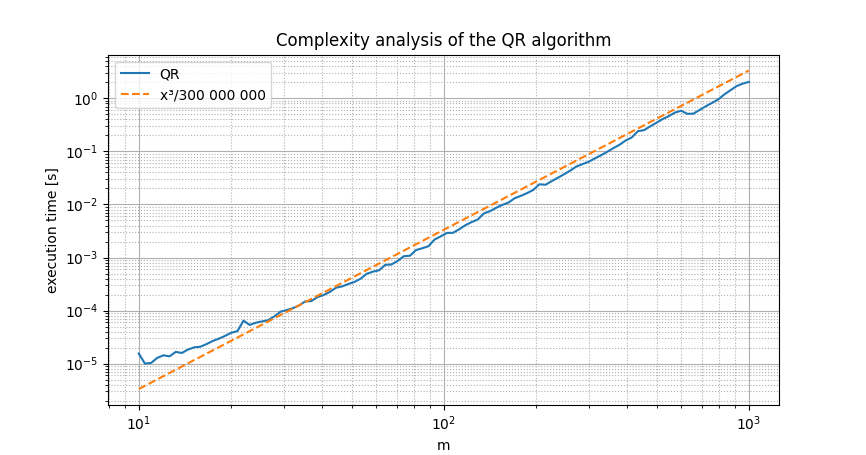
\includegraphics[scale=0.6]{images/perf.png}
\end{figure}

\section{Approximation par des B-splines}

Voici quelques exemples d'approximation par des b-splines sur des points en coeur. Nous voyons que plus on $n$ s'approche de $m$, plus l'approximation est précise et rafinée, mais à partir d'un certain seuil (plus ou moins 9/10 de m), des points de contrôle commencent à se placer loin de la figure, et quand m = n, il y a un point qui est très très éloigné.

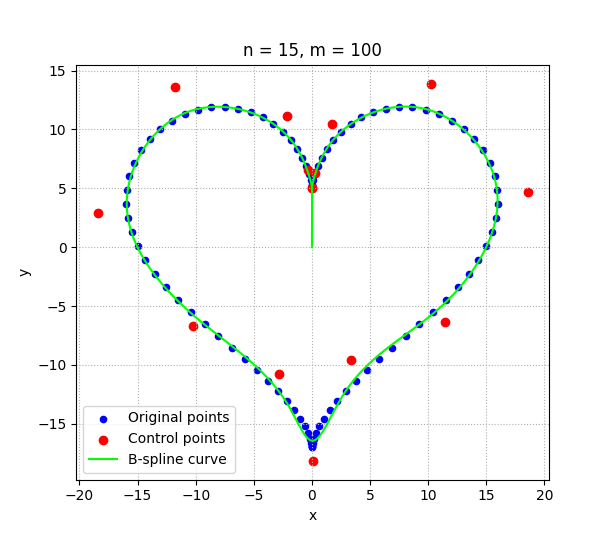
\includegraphics[scale=0.32]{images/coeur1.png}
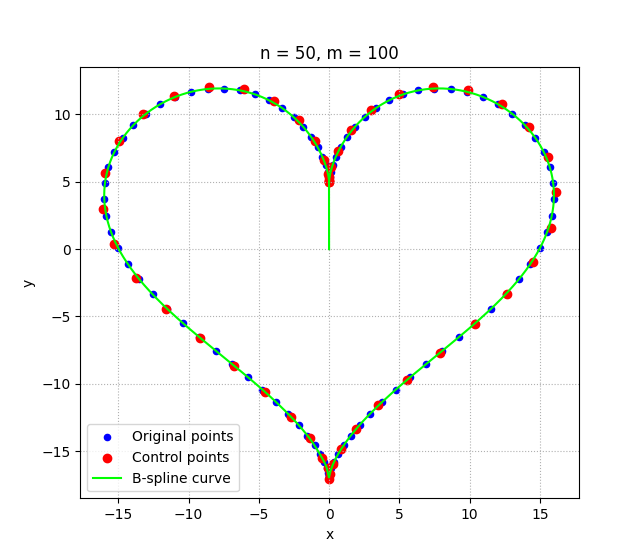
\includegraphics[scale=0.31]{images/coeur2.png}
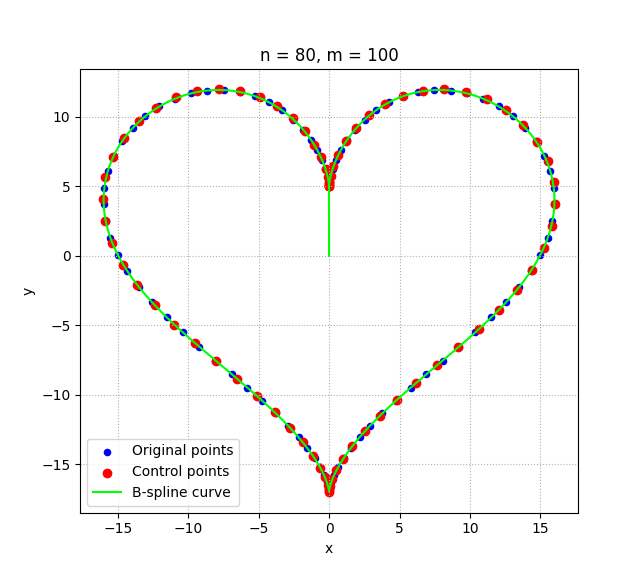
\includegraphics[scale=0.3]{images/coeur3.png}
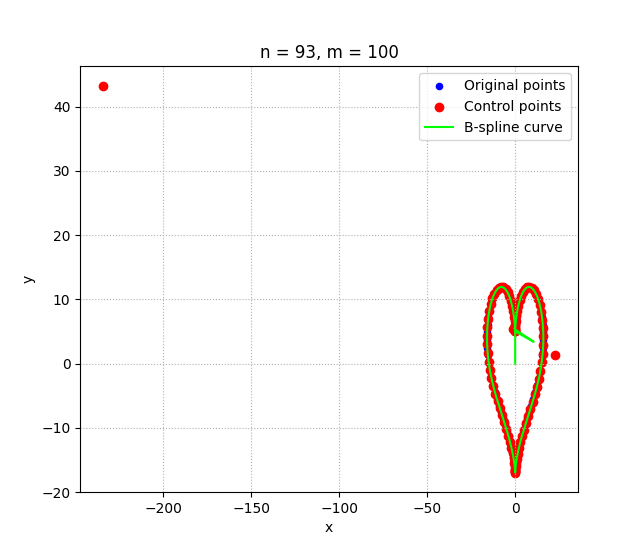
\includegraphics[scale=0.3]{images/coeur4.png}
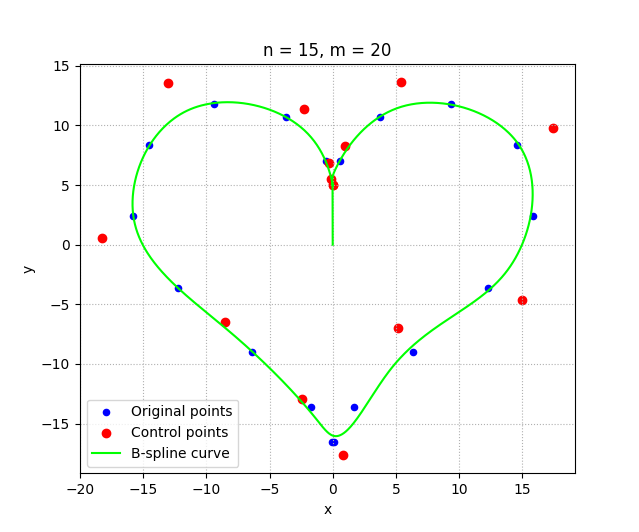
\includegraphics[scale=0.31]{images/coeur5.png}
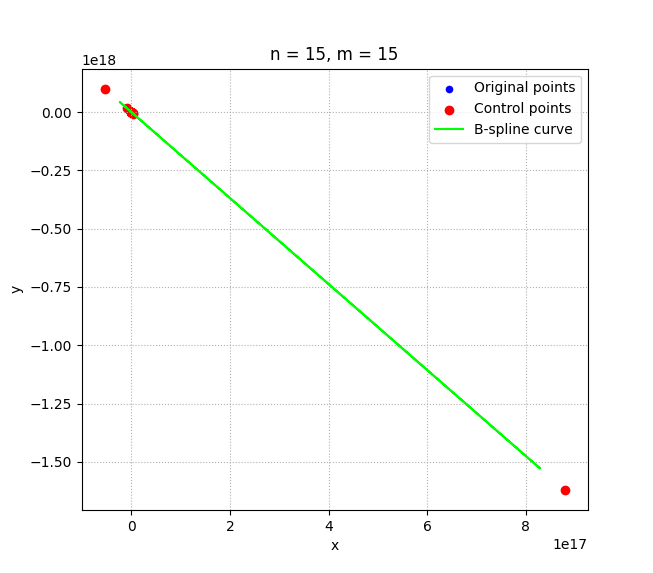
\includegraphics[scale=0.3]{images/coeur6.png}

Ici nous pouvons voir une tentative de dessin d'une tortue avec 684 points fournis, et avec respectivement 100 et 300 points de contrôle.

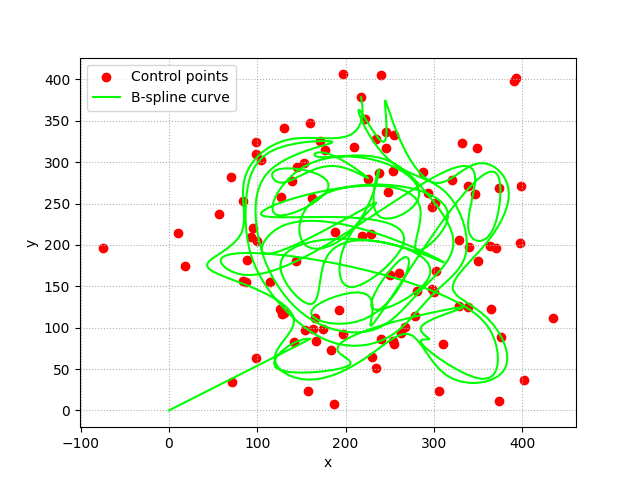
\includegraphics[scale=0.3]{images/turtle.png}
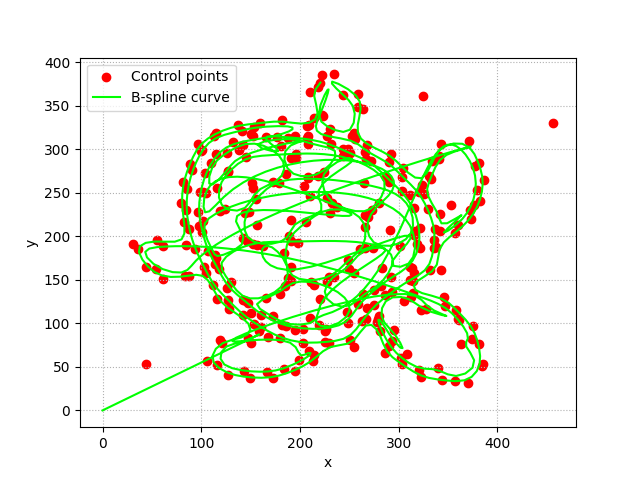
\includegraphics[scale=0.3]{images/turtle2.png}

\end{document}